\documentclass[xcolor=table,xcolor=dvipsnames,handout]{beamer}

\mode<presentation> {

% The Beamer class comes with a number of default slide themes
% which change the colors and layouts of slides. Below this is a list
% of all the themes, uncomment each in turn to see what they look like.

%\usetheme{default}
%\usetheme{AnnArbor}
%\usetheme{albatross}
%\usetheme{Antibes}
%\usetheme{Bergen}
%\usetheme{Berkeley}
%\usetheme{Berlin}
%\usetheme{Boadilla}
%\usetheme{CambridgeUS}
%\usetheme{Copenhagen}
%\usetheme{Darmstadt}
%\usetheme{Dresden}
%\usetheme{Frankfurt}
%\usetheme{Goettingen}
%\usetheme{Hannover}
%\usetheme{Ilmenau}
%\usetheme{JuanLesPins}
%\usetheme{Luebeck}
\usetheme{Madrid}
%\usetheme{Malmoe}
%\usetheme{Marburg}
%\usetheme{Montpellier}
%\usetheme{PaloAlto}
%\usetheme{Pittsburgh}
%\usetheme{Rochester}
%\usetheme{Singapore}
%\usetheme{Szeged}
%\usetheme{Warsaw}

% As well as themes, the Beamer class has a number of color themes
% for any slide theme. Uncomment each of these in turn to see how it
% changes the colors of your current slide theme.

% \usecolortheme{dracula}
%\usecolortheme{albatross}
%\usecolortheme{beaver}
%\usecolortheme{beetle}
%\usecolortheme{crane}
%\usecolortheme{dolphin}
%\usecolortheme{dove}
%\usecolortheme{fly}
%\usecolortheme{lily}
%\usecolortheme{orchid}
%\usecolortheme{rose}
%\usecolortheme{seagull}
%\usecolortheme{seahorse}
%\usecolortheme{whale}
%\usecolortheme{wolverine}

%\setbeamertemplate{footline} % To remove the footer line in all slides uncomment this line
%\setbeamertemplate{footline}[page number] % To replace the footer line in all slides with a simple slide count uncomment this line

%\setbeamertemplate{navigation symbols}{} % To remove the navigation symbols from the bottom of all slides uncomment this line
}
\setbeamertemplate{frametitle continuation}{}
  \setbeamertemplate{enumerate items}[default]
\setbeamertemplate{itemize items}{--}

\setbeamercovered{invisible}
\setbeamercovered{again covered={\opaqueness<1->{30}}}
\setbeamercovered{transparent}

%!TEX root = main.tex

\usepackage[in]{fullpage}
\usepackage[dvipsnames]{xcolor}
% \usepackage[backend=bibtex]{biblatex}

\usepackage[
bookmarksopen,
bookmarksdepth=2,
% linkcolor=black,
breaklinks=true,
colorlinks=true,
citecolor=red,
urlcolor=blue
]{hyperref}

\usepackage{authblk}
\usepackage{blindtext}
\usepackage{wrapfig}
\setlength{\parskip}{.5em}
\usepackage{svg}

\usepackage{changepage}
\usepackage{extarrows} 

\usepackage[center]{titlesec}
\titlelabel{\thetitle. }


\usepackage{titling}
\usepackage{breqn}
\settowidth{\thanksmarkwidth}{*}
\setlength{\thanksmargin}{-\thanksmarkwidth}
% \usepackage{fancyhdr}
\usepackage{authblk}
\usepackage{xfrac}


\usepackage{appendix}
\usepackage{soul}

\usepackage{inconsolata}
\usepackage{graphicx}% Include figure files
\usepackage{subcaption}% Include figure files

\usepackage{algorithm}
\newcommand{\algcaption}[1]{\caption{#1}}

% \usepackage[ruled,vlined,linesnumbered]{algorithm2e}
\usepackage{algpseudocode}

\graphicspath{{figs/}{figs/1/}{figs/2/}{figs/3/}{figs/4/}{figs/5/}{figs/6/}{figs/7/}} %Setting the graphicspath

\usepackage{bm}% bold m
\usepackage{float}
\usepackage{tabularx}
\usepackage{amsfonts}
\usepackage{amssymb}
\usepackage{amsmath}
\usepackage{amsthm}
\usepackage{mathtools}
\usepackage{bm}
\usepackage{tikz}
\usepackage{enumerate}
\usepackage{mathtools}
\usepackage{multirow}
\usepackage{mdframed}

\usepackage{silence}
  % \WarningFilter*{mdframed}{You got a bad break(mdframed) }
  \WarningFilter*{latex}{Label `' multiply defined}
  \WarningFilter*{latex}{There were multiply-defined labels.}
\WarningsOff

\usepackage{mathtools}
\usepackage{listings}

\usepackage[inline]{enumitem}
\setlist{nosep} % or \setlist{noitemsep} to leave space around whole list



%!TEX root = main.tex

\let\oldtextbf\textbf
\renewcommand{\textbf}[1]{\oldtextbf{\boldmath #1}}



\renewcommand\labelitemi{--}



\newtheorem{theorem}{Theorem}[section]
\newtheorem{corollary}{Corollary}[theorem]
\newtheorem{lemma}[theorem]{Lemma}


% \theoremstyle{definition}
\newtheorem{definition}{Definition}[section]
\newtheorem{example}{Example}[section]


\newcommand{\eq}{\Leftrightarrow}

\newcommand{\floor}[1]{\left\lfloor #1 \right\rfloor}
\newcommand{\ceil}[1]{\left\lceil #1 \right\rceil}


\renewcommand{\vec}[1]{\bm{#1}}


% \newcommand{\norm}[1]{\lvert #1 \rvert}
\newcommand{\norm}[1]{\left\lvert#1\right\rvert}
\renewcommand{\Pr}[1]{\text{Pr}\left[#1\right]}
\newcommand{\lp}[1]{\left(#1\right)}
\newcommand{\lb}[1]{\left[#1\right]}
\newcommand{\lbr}[1]{\left\{#1\right\}}
\newcommand{\lng}[1]{\left\langle#1\right\rangle}

\newcommand{\summ}[2]{\sum_{#1}^{#2}}
\newcommand{\prodd}[2]{\prod_{#1}^{#2}}


\newcommand*{\qedb}{\null\nobreak\hfill\ensuremath{\blacksquare}}%
\newcommand{\xor}{\oplus}


\newcommand{\negl}{\textsf{negl}}

% \newcommand{\getsrv}{\stackrel{\$}{\gets}}
\newcommand{\getsrv}{\xleftarrow{\text{\tiny{\$}}}}


\newcommand{\nin}{\notin}
% \setlength\parindent{0pt}
\renewcommand{\O}{\mathcal{O}}
\newcommand{\X}{\mathcal{X}}
\newcommand{\W}{\mathcal{W}}
\newcommand{\Y}{\mathcal{Y}}
\newcommand{\I}{\mathcal{I}}
\newcommand{\E}{\mathcal{E}}
\newcommand{\ID}{\mathcal{ID}}
\newcommand{\R}{\mathbb{R}}
\newcommand{\U}{\mathcal{U}}
\newcommand{\Z}{\mathbb{Z}}
\newcommand{\T}{\mathbb{T}}
\renewcommand{\S}{\mathbb{S}}
\newcommand{\G}{\mathbb{G}}
\newcommand{\Gdh}{\mathbb{G}_{\textsc{dh}}}
\newcommand{\N}{\mathcal{N}}
\newcommand{\NP}{\mathcal{NP}}
\renewcommand{\P}{\mathcal{P}}
\newcommand{\C}{\mathcal{C}}
\newcommand{\A}{\mathbb{A}}
\newcommand{\F}{\mathbb{F}}
\newcommand{\K}{\mathcal{K}}
\newcommand{\M}{\mathcal{M}}
\newcommand{\of}{\subseteq}
\newcommand{\fo}{\supseteq}
\newcommand{\nof}{\subsetneq}
\newcommand{\nfo}{\supsetneq}
\newcommand{\emp}{\emptyset}
\newcommand{\val}{\text{val}}
\newcommand{\spn}{\text{span}}
\newcommand{\rank}{\text{rank}}
\newcommand{\argmax}{\text{argmax}}
\renewcommand{\st}{s\text{-}t}
\newcommand{\ST}{S\text{-}T}

\newcommand{\twae}{\text{twae}}
\newcommand{\awae}{\text{awae}}
\newcommand{\jwae}{\text{jwae}}
\newcommand{\relu}{\text{ReLU}}
\newcommand{\enc}{\text{Enc}}
\newcommand{\dec}{\text{Dec}}
\newcommand{\sh}{\text{Sh}}

\newcommand{\Yb}{\bar{Y}}
\newcommand{\sm}{\setminus}


\renewcommand{\mod}{\ \mathrm{mod}\ }


\renewcommand{\And}{\textbf{and} }

 \newenvironment{protocol}[1]% environment name
{% begin code
  \par\vspace{\baselineskip}\noindent
\begin{mdframed}
    \noindent\textbf{\emph{#1}:}
    \begin{adjustwidth*}{1cm}{1cm} 
    \setlength{\parindent}{0pt}
    }
    % \parindent0pt
{% end code
  \end{adjustwidth*}
  \end{mdframed}  
  \ignorespacesafterend
} 

\lstset{
  basicstyle=\ttfamily,
}

\makeatletter                                                              
% \SetAlgorithmName{Protocol}{protocol}{List of Protocols}
\renewcommand*{\listalgorithmcfname}{List of Protocols}
\renewcommand*{\algorithmcfname}{Protocol}
\renewcommand*{\algorithmautorefname}{protocol}
% \renewcommand{\ALG@name}{Protocol}                                             
% \makeatother
% \renewcommand{\algorithmicforall}{\textbf{for each}}

% \makeatletter
% \newcommand{\LINEFORALL}[3][default]{%
%   \ALC@it\algorithmicforall\ #2\ \algorithmicdo%
%   \ALC@com{#1}\ #3%
% }
% \newcommand{\LINEENDFOR}{\ALC@it\algorithmicendfor}
% \makeatother
\newcommand{\received}{\text{received}}



\newenvironment<>{varblock}[2][\textwidth]{%
  \setlength{\textwidth}{#1}
  \begin{actionenv}#3%
    \def\insertblocktitle{#2}%
    \par%
    \usebeamertemplate{block begin}}
  {\par%
    \usebeamertemplate{block end}%
  \end{actionenv}}

\newenvironment<>{varexamp}[2][\textwidth]{%
  \setlength{\textwidth}{#1}
  \begin{actionenv}#3%
    \def\insertblocktitle{#2}%
    \par%
    \usebeamertemplate{block example begin}}
  {\par%
    \usebeamertemplate{block example end}%
  \end{actionenv}}





\AtBeginSection[]{
  \begin{frame}
  \vfill
  \centering
  \begin{beamercolorbox}[sep=8pt,center,shadow=true,rounded=true]{title}
    \usebeamerfont{title}\insertsectionhead\par%
  \end{beamercolorbox}
  \vfill
  \end{frame}
}






\title[The Apple PSI System]{The Apple PSI System \\\cite{bhowmick2021apple}
} % The short title appears at the bottom of every slide, the full title is only on the title page

\author[A. Baccarini]{Alessandro Baccarini} % Your name
\institute[University at Buffalo] % Your institution as it will appear on the bottom of every slide, may be shorthand to save space
{
University at Buffalo \\ % Your institution for the title page
\medskip
\texttt{anbaccar@buffalo.edu} % Your email address
}
\date{\today} % Date, can be changed to a custom date

\begin{document}

\begin{frame}
\titlepage % Print the title page as the first slide
\end{frame}


\begin{frame}[c]
  \frametitle{Table of Contents}

\tableofcontents  
\end{frame}



\section{Motivations} % (fold)
\label{sec:motivations}

\begin{frame}[c]
  \frametitle{Why?}
 \begin{itemize}
    \item August 2021 -- Apple unveils plans for new Child Sexual Abuse Material (CSAM) detection system.
    \pause
    \item Designed to automatically detect known CSAM images stored in iCloud, and report the users to authorities.
    \pause
    \item Aimed to be packaged with iOS 15 and iPadOS 15.
    \pause
    \item Very poorly received in media and tech communities.

\begin{figure}
    \begin{overprint}
    \onslide<5>\centering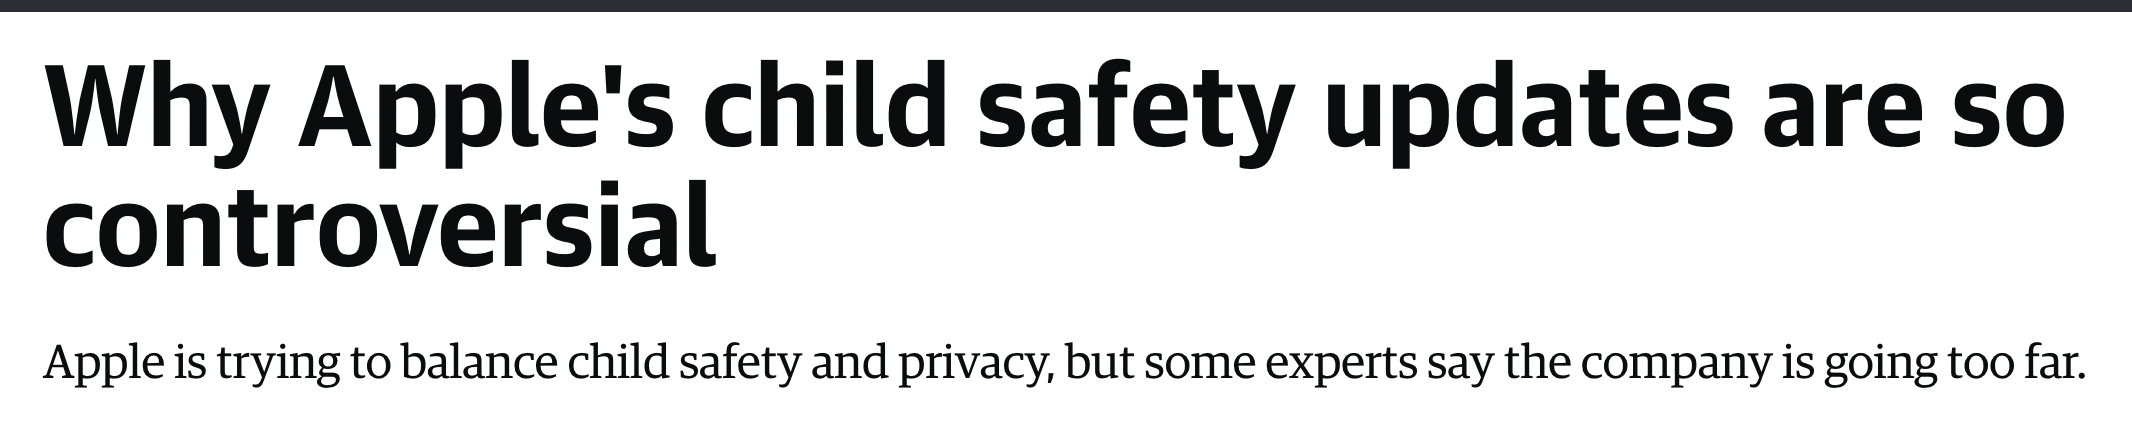
\includegraphics[width=0.8\textwidth]{a1}
    \onslide<6>\centering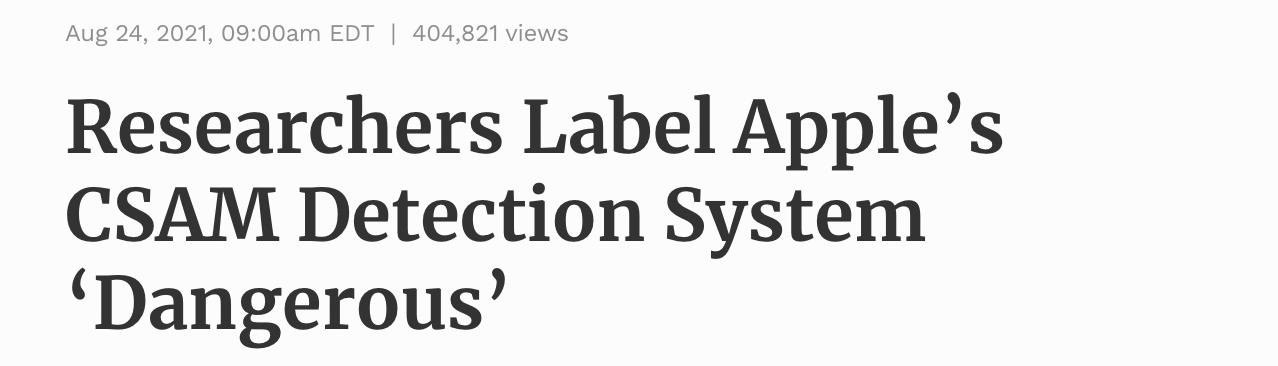
\includegraphics[width=0.8\textwidth]{a2}
    \onslide<7->\centering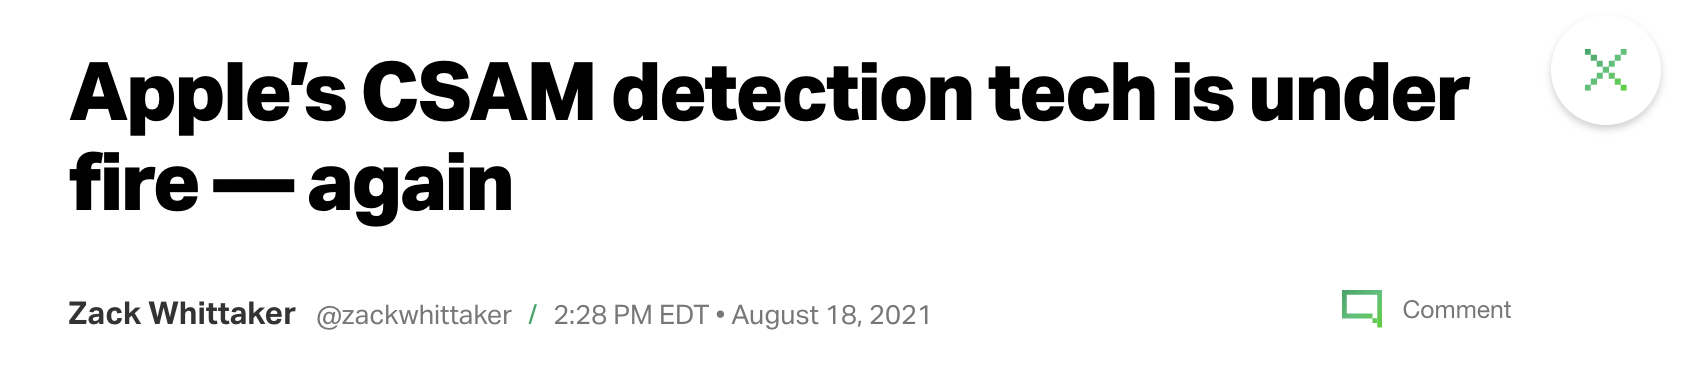
\includegraphics[width=0.8\textwidth]{a3}
    \end{overprint}\end{figure}
    \item<8> September 2021 -- Apple postpones rollout indefinitely.
    \pause

  \end{itemize} 
\end{frame}


{
\setbeamercovered{transparent} 

\begin{frame}[c]
  \frametitle{What security goals do ``we'' want?}
  \begin{itemize}
    \pause

  \item Server cannot recover the user's matched photos without exceeding some threshold.
    \pause
  \item False positives are impossible.
    \pause
  \item No information is learned about non-matched images.
    \pause
  \item User cannot learn any information from the CSAM database.
    \pause
  \item User cannot identify which images were flagged as CSAM by the system.
\end{itemize}
\end{frame}
}

\begin{frame}[c]
  \frametitle{NeuralHash}
  \begin{itemize}
    \item Different from our standard notion of hash functions.
    \pause
    \item Insensitive to small perturbations (cropping, rotation, mirroring, watermarking).
\begin{figure}[htbp]
\only<2>{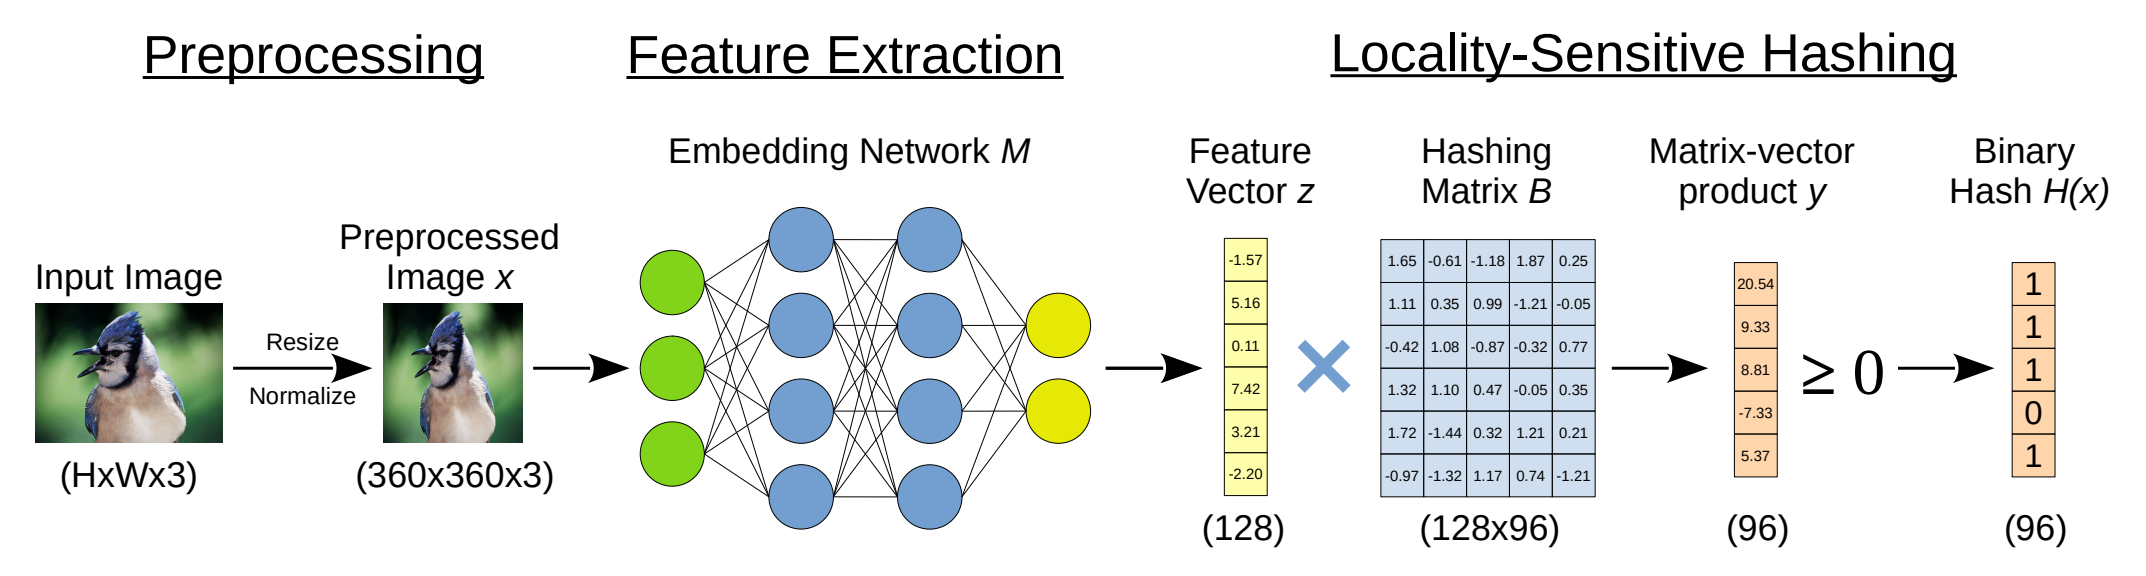
\includegraphics[width=0.95\textwidth]{nn_hash}
\cite{struppek2021learning}
}
\end{figure}
  \end{itemize}
\end{frame}


{
\setbeamercovered{} 
\begin{frame}[c,fragile]

  \frametitle{NeuralHash}

  \begin{itemize}


    \item Contains some collision-related issues \cite{athalyeNeuralHashCollider2021}...


    \pause
  \end{itemize}

\begin{figure}[htbp]
  % \centering
  \only<2->{\raisebox{-.35\height}{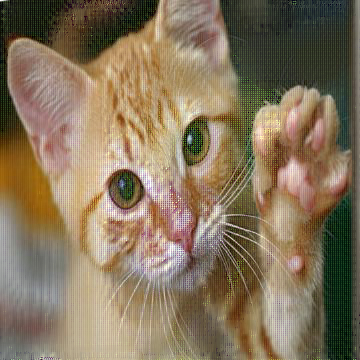
\includegraphics[width=0.25\textwidth]{cat}} {\Huge{ $\stackrel{?}{=}$ }}}
  \only<2->{\raisebox{-.35\height}{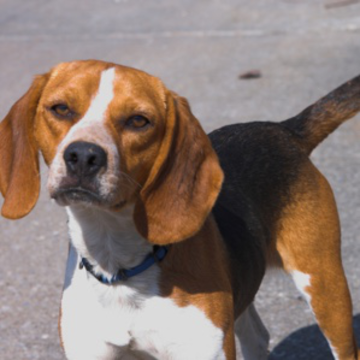
\includegraphics[width=0.25\textwidth]{dog}}}
\end{figure}

\pause
\begin{lstlisting}[language=Python,keywordstyle=\color{red}]
    $ python nnhash.py cat.png
    59a34eabe31910abfb06f308
    $ python nnhash.py dog.png
    59a34eabe31910abfb06f308
\end{lstlisting}
\end{frame}
}



\begin{frame}[c]
  \frametitle{A Crash Course in Private Set Intersection (PSI)}
  \begin{itemize}
    \item Let $\U$ be the universe of all possible image hashes.
    \pause
    \item $X \of \U$ is set of image hashes we want to match against, stored on the server.
    \pause
    \item A client has a list of $m$ triples 
    \begin{align*}
      \bar{Y} = \lp{\lp{y_1, id_1, ad_1} , \dots   \lp{y_m, id_m, ad_m}} \in \lp{\U \times \ID \times \D}^m,
    \end{align*}
    where $y \in \U$ is the hash of an image, a unique identifier $id \in \ID$, and some associated data $ad \in \D$.
    \pause
    \item When the protocol terminates, the server learns the identifiers and associated data of the intersection of $\bar{Y}$ and $X$, namely $id \lp{\bar{Y} \cap X}$

  \end{itemize}
\end{frame}


{
\setbeamercovered{again covered={\opaqueness<1->{30}}}
\begin{frame}[c]
  \frametitle{Two PSI Protocols}
  
  \begin{block}{Threshold PSI-AD}
    Add a threshold parameter $t$, such that if $\norm{id \lp{\bar{Y} \cap X}} \leq t$, the server learns only the $id$'s. If $\norm{id \lp{\bar{Y} \cap X}} > t$, then the server learns the associated data for all identifiers in the intersection.
  \end{block}
\pause

  \begin{block}{Fuzzy Threshold PSI-AD}<2>
   Extension of prior scheme, but adds ``synthetic matches'' so the server does not know the number of matches in the intersection before the threshold $t$ is exceeded.
  \end{block}
  \pause
\end{frame}}

{
\setbeamercovered{transparent}
\section{Protocol Description} % (fold)
\label{sec:protocol_description}

\begin{frame}[c]
  \frametitle{Server Setup}
  
  \begin{enumerate}
    \item Remove any duplicates from $X$, and let $n = \norm{X}$.
  \pause
    \item Construct a hash table $T$:
  \pause
    \begin{itemize}
      \item Let $n' \geq n$ be the size of the table (minimize collisions).
      \item Choose hash function $h : \U \to \lbr{1,\dots,n'}$ (SHA256 modulo $n'$).
      \item Insert elements of $X$ into $T$, each cell should have at most one element.
    \end{itemize}
  \pause
    \item Choose a random nonzero $\alpha \in \F_q$, compute $L = G^\alpha \in \G$, where $\G$ is a DH group modulo prime $p$ (2048-bit) with a fixed generator $G = 2$.
  \pause
    \item For $i = 1$ to $n'$ do:
  \pause
    \begin{itemize}
      \item If $T[i]$ is non-empty, set $P_i = {H(T[i])^{\alpha}} \in \G$, where $T[i] \in X \of \U$, and $H: \U \to \G$ (SHA256 modulo $p$).
      \item  If $T[i]$ is empty, choose a random $P_i \in \G$.
    \end{itemize}
  \pause
    \item set $pdata = \lp{L, P_1, \dots, P_{n'}}$.
  \end{enumerate}
  
\end{frame}



\begin{frame}[c]
  \frametitle{Client Setup}
  \begin{enumerate}
    \item Obtain $pdata$ from the server.
  \pause
    \item Generate keys:
    \begin{itemize}
  \pause
      \item $adkey \gets \K'$ for  encryption scheme $\lp{\enc, \dec}$.
      \begin{itemize}
        \item We use AES128-GCM for its ``random key robustness'' property.
        \item $Dec(Enc(k,m), k')$ should fail, where $k \neq k'$ are independent random keys.
      \end{itemize}
  \pause
      \item $fkey \gets \K''$ for the PRF $F: \K'' \times \ID \to \F_{\sh}$.
  \pause
      \item Initialize threshold \emph{Shamir secret sharing} for $adkey$:
      \begin{align*}
      f(x) = a_0 + a_1x + a_2x + \dots + a_{t}x^{t},
      \end{align*}
      where $a_0 = adkey$ is the secret. Reconstruction involves Lagrange interpolation.
    \end{itemize}
  \end{enumerate}
  
  
\end{frame}




\begin{frame}[c]
  \frametitle{Client Voucher Generation on Input Triple  $(y, id, ad)$}
  \begin{enumerate}

     \item Encrypt $ad$ as $adct \gets \enc \lp{adkey, ad},$ and all $adct$ must be the same length.
  \pause
     \item Compute $x = F(fkey, id) \in \F_{\sh}$.

  \pause
     \item Generate a share $sh = \lp{x, f(x)} \in \F_{\sh}$ of $adkey$ (guarantees duplicate triples with the same $id$ will produce the same $sh$).


  \pause
     \item Choose a random key $rkey \gets \K'$ and compute $rct \gets \enc \lp{rkey, \lp{adct, sh}}$.%concatenation?

    \seti
   \end{enumerate} 
\end{frame}
    

\begin{frame}[c]
  \frametitle{Client Voucher Generation on Input Triple  $(y, id, ad)$}
  \begin{enumerate}
    \conti

     \item Compute $w = h(y) \in \lbr{1,\dots,n'}$.
  \pause
     \item Sample random  $\beta, \gamma \in \F_q$, and use $P_w,L$ from $pdata$ to compute:
     \begin{align*}
     Q = H(y)^{\beta} \cdot G^{\gamma} \text{ and } S = P_w^{\beta} \cdot L^{\gamma},
     \end{align*}
     where if $y = T[w]$, then $P_w = H(y)^{\alpha}$ and $S = Q^{\alpha}$ (DH random self reduction).
  \pause
  \item Compute $ct \gets \enc \lp{H'(S), rkey},$ where $H' : \G \to \K'$ (HKDF with SHA256).
  \pause
     \item Send $voucher = (id, Q, ct, rct)$ to the server.
   \end{enumerate} 
  
\end{frame}


\begin{frame}[c]
  \frametitle{Server Voucher Processing}
  \begin{enumerate}
    \item Initialize empty set $SHARES$ and an empty list $IDLIST$.
  \pause
    \item For each voucher $(id, Q, ct, rct)$ received, do:
  \pause
    \begin{itemize}
      \item Append $id$ to IDLIST.
      \item Compute $\hat{S} = Q^{\alpha} \in \G$, 
      \item Set $rkey = \dec (H'(\hat{S}), ct)$.
      \item Set $(adct, sh) = \dec (rkey, rct)$.
  \pause
      \item If either decryptions ``fails'', $y$ is a non-match, and ignore the voucher. 
      \item Otherwise, we found a match and add $(id, adct, sh)$ to $SHARES$.
    \end{itemize}


    \seti
   \end{enumerate} 
\end{frame}
    

\begin{frame}[c]
  \frametitle{Server Voucher Processing}
  \begin{enumerate}
    \conti



    \item Let $t'$ denote the number of \emph{unique} shares in $SHARES$, and $t'$ should equal the size of $id (\bar{Y} \cap X)$. 
  \pause
    \begin{itemize}
      \item If $t' \leq t$, let $OUTSET$ be the set of identifiers in $SHARES$.
      \item If $t' > t$, do:
  \pause
      \begin{itemize}
        \item Use $(t+1)$ shares to reconstruct $adkey \in \K'$.
        \item Initialize $OUTSET = \lbr{\emp}$.
        \item For each triple $(id, adct, sh) \in SHARES$, compute $ad = \dec (adkey, adct)$. If it fails, discard the voucher. Otherwise, add $(id,ad )$ to $OUTLIST$.
      \end{itemize}
  \pause
      \item Output $IDLIST$ and $OUTSET$.
    \end{itemize}
  \end{enumerate}
  
\end{frame}


}


\begin{frame}[c]
  \frametitle{(Brief) Discussion}
\begin{itemize}
    \item Protocol is correct if the client and server adhere to the protocol (proof omitted for obvious reasons).
  \pause
    \item Using ``simpler'' constructions guarantees the same level of security as the original protocol (potentially for the price of degraded performance).
  \pause
    \item Construction naturally extends to ftPSI-AD, requires novel primitives.
    \begin{itemize}
  \pause
      \item Detectable hash functions, hashing to elliptic curves,~etc.
    \end{itemize}
  \end{itemize}  
\end{frame}


\section{Conclusions} % (fold)
\label{sec:conclusions}


\begin{frame}[c]
  \frametitle{Conclusions}
  \begin{itemize}
    \item Presented Apple's PSI system for CSAM detection.
    \pause
    \item The protocol is cryptographically sound, and meets the security goals specified earlier.
  \end{itemize}
\end{frame}


 \begin{frame}[c]
  \frametitle{Conclusions}
  \begin{itemize}   
    \item So why is something like this still bad?
    \pause
    \item What are the implications of this system?
  \end{itemize}
   
\end{frame}



\begin{frame}[allowframebreaks]
\frametitle{References} 
\footnotesize{
\bibliographystyle{apalike} 
\bibliography{psi-refs} 
}
\end{frame}

\begin{frame}[c]

\begin{center}
\Huge Thank you! \\ 
\vspace{1.0em}
\Large Questions?
\end{center}
\end{frame}

\appendix 

\end{document} 